\scanpage{113}
trois pts marqués $0,1,\infty$, avec le groupe d'autom. holomorphes $\unsure{\mathfrak S_3|\mathfrak G_3}$, il y a une métrique positive \deleted{\unsure{invariante}} \inserted{homogène} unique invariante par $\unsure{\mathfrak S_3|\mathfrak G_3}$. On va prendre un système de disques $D_i$ ($i\in\{0,1,\infty\}$) \uline{stable par} $\unsure{\mathfrak S_3|\mathfrak G_3}$, et \deleted{formé} limités par des cercles de centre $i$ (au sens de la structure riemannienne) --- il revient au $=$ de se donner en \uline{un} des $i$, disons $i=\infty$, un cercle \inserted{de centre $i$} qui soit \uline{invariant$^*$ par la transposition des deux autres}, et de plus \uline{assez petit} pour que ses \inserted{trois} transformés par $\unsure{\mathfrak S_3|\mathfrak G_3}$ mod le sous-groupe de stabilité, définissent des disques mutuellement disjoints.
\margin{$^*$ c'est automatique}

On prendra comme modèle riemannien une $2$-sphère \inserted{euclidienne} \inserted{orientée}, \deleted{$\unsure{\Sigma=\Sigma_I}$, \unsure{de rayon} $=1$,} $\Sigma=\Sigma_I$, de rayon $1$, un grand cercle fixé, \inserted{$\unsure{\Sigma_{\mathbb R}}$} et \deleted{trois points \unsure{de celui-ci}} \inserted{une} \deleted{deux cercles disjoints dessus} partie $I$ dessus formant un triangle équilatéral inscrit --- le choix des cercles dépend d'un paramètre $0\leq\rho\leq1$ (son rayon rectiligne).
\figure{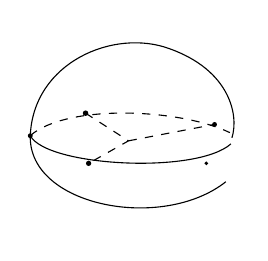
\begin{tikzpicture}[x=1.3cm,y=1.3cm]
\draw (-1,0) .. controls (-.97,.72) and (-.18,1.05) .. (.36,.85) .. controls (.95,.64) and (1.04,.20) .. (.97,-.02);
\draw (-1,0) .. controls (-1.02,-.69) and (.29,-.94) .. (.91,-.45);
\draw (-1,0) .. controls (-.84,-.30) and (.62,-.38) .. (.96,-.08);
\draw[dashed] (-1,0) .. controls (-.65,.31) and (.45,.27) .. (.95,.03);
\draw[dashed] (-.46,.22)--(-.04,-.05)--(-.43,-.27);
\draw[dashed] (-.04,-.05)--(.80,.11);
\fill (-1,0) circle (.024);\fill (-.46,.22) circle (.027);\fill (-.43,-.27) circle (.026);\fill (.80,.11) circle (.024);\fill (.72,-.27) circle (.019);
\end{tikzpicture}}
\deleted{Pour} tout $i\in I$, le cercle $\unsure{\Gamma|T}_{i\rho}\deleted{^{\unsure{\rho}}}$ admet deux pts \deleted{\unsure{marqués}} sur l'équateur, \deleted{\unsure{canoniquement marqués}}
\figure{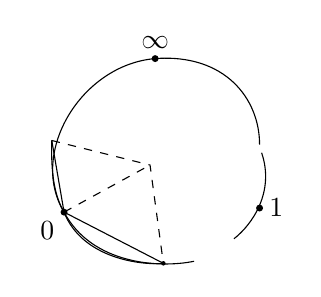
\begin{tikzpicture}[x=1.3cm,y=1.3cm]
\draw (-.89,-.50) .. controls (-1.24,.08) and (-.72,.94) .. (0,1) .. controls (.68,1.05) and (1.02,.61) .. (1.02,.16);
\draw (1.04,.08) .. controls (1.17,-.30) and (.95,-.62) .. (.77,-.76);
\draw (-.89,-.50) .. controls (-.62,-1.01) and (.04,-1.05) .. (.38,-.98);
\draw (-1.01,.20)--(-.89,-.50);
\draw (-1.01,.20) .. controls (-1.02,-.13) and (-.98,-.35) .. (-.89,-.50);
\draw (-.89,-.50)--(.08,-1);
\draw (-.89,-.50) .. controls (-.71,-.96) and (-.12,-1.02) .. (.08,-1);
\draw[dashed] (-1.01,.20)--(-.05,-.04)--(.08,-1);
\draw[dashed] (-.89,-.50)--(-.05,-.04);
\fill (0,1) circle (.034) node[above] {$\infty$};
\fill (1.02,-.46) circle (.034) node[right] {$1$};
\fill (-.89,-.50) circle (.034) node[below left] {$0$};
\fill (.08,-1) circle (.022);
\end{tikzpicture}}
\mspage{112}
